%----------------------------------------------------------------------------------------
%	PACKAGES AND OTHER DOCUMENT CONFIGURATIONS
%----------------------------------------------------------------------------------------

\documentclass{article}
\usepackage{mathtools}
\usepackage{float}

%----------------------------------------------------------------------------------------
%	PACKAGES AND OTHER DOCUMENT CONFIGURATIONS
%----------------------------------------------------------------------------------------

\usepackage{amsmath,amsfonts,stmaryrd,amssymb} % Math packages

\usepackage{enumerate} % Custom item numbers for enumerations

\usepackage[ruled]{algorithm2e} % Algorithms

\usepackage[framemethod=tikz]{mdframed} % Allows defining custom boxed/framed environments

\usepackage{listings} % File listings, with syntax highlighting
\lstset{
	basicstyle=\ttfamily, % Typeset listings in monospace font
}

%----------------------------------------------------------------------------------------
%	DOCUMENT MARGINS
%----------------------------------------------------------------------------------------

\usepackage{geometry} % Required for adjusting page dimensions and margins

\geometry{
	paper=a4paper, % Paper size, change to letterpaper for US letter size
	top=2.5cm, % Top margin
	bottom=3cm, % Bottom margin
	left=2.5cm, % Left margin
	right=2.5cm, % Right margin
	headheight=14pt, % Header height
	footskip=1.5cm, % Space from the bottom margin to the baseline of the footer
	headsep=1.2cm, % Space from the top margin to the baseline of the header
	%showframe, % Uncomment to show how the type block is set on the page
}

%----------------------------------------------------------------------------------------
%	FONTS
%----------------------------------------------------------------------------------------

\usepackage[utf8]{inputenc} % Required for inputting international characters
\usepackage[T1]{fontenc} % Output font encoding for international characters

\usepackage{newtxtext} % Use the XCharter fonts

%----------------------------------------------------------------------------------------
%	COMMAND LINE ENVIRONMENT
%----------------------------------------------------------------------------------------

% Usage:
% \begin{commandline}
%	\begin{verbatim}
%		$ ls
%		
%		Applications	Desktop	...
%	\end{verbatim}
% \end{commandline}

\mdfdefinestyle{commandline}{
	leftmargin=10pt,
	rightmargin=10pt,
	innerleftmargin=15pt,
	middlelinecolor=black!50!white,
	middlelinewidth=2pt,
	frametitlerule=false,
	backgroundcolor=black!5!white,
	frametitle={Command Line},
	frametitlefont={\normalfont\sffamily\color{white}\hspace{-1em}},
	frametitlebackgroundcolor=black!50!white,
	nobreak,
}

% Define a custom environment for command-line snapshots
\newenvironment{commandline}{
	\medskip
	\begin{mdframed}[style=commandline]
}{
	\end{mdframed}
	\medskip
}

%----------------------------------------------------------------------------------------
%	FILE CONTENTS ENVIRONMENT
%----------------------------------------------------------------------------------------

% Usage:
% \begin{file}[optional filename, defaults to "File"]
%	File contents, for example, with a listings environment
% \end{file}

\mdfdefinestyle{file}{
	innertopmargin=1.6\baselineskip,
	innerbottommargin=0.8\baselineskip,
	topline=false, bottomline=false,
	leftline=false, rightline=false,
	leftmargin=2cm,
	rightmargin=2cm,
	singleextra={%
		\draw[fill=black!10!white](P)++(0,-1.2em)rectangle(P-|O);
		\node[anchor=north west]
		at(P-|O){\ttfamily\mdfilename};
		%
		\def\l{3em}
		\draw(O-|P)++(-\l,0)--++(\l,\l)--(P)--(P-|O)--(O)--cycle;
		\draw(O-|P)++(-\l,0)--++(0,\l)--++(\l,0);
	},
	nobreak,
}

% Define a custom environment for file contents
\newenvironment{file}[1][File]{ % Set the default filename to "File"
	\medskip
	\newcommand{\mdfilename}{#1}
	\begin{mdframed}[style=file]
}{
	\end{mdframed}
	\medskip
}

%----------------------------------------------------------------------------------------
%	NUMBERED QUESTIONS ENVIRONMENT
%----------------------------------------------------------------------------------------

% Usage:
% \begin{question}[optional title]
%	Question contents
% \end{question}

\mdfdefinestyle{question}{
	innertopmargin=1.2\baselineskip,
	innerbottommargin=0.8\baselineskip,
	roundcorner=5pt,
	nobreak,
	singleextra={%
		\draw(P-|O)node[xshift=1em,anchor=west,fill=white,draw,rounded corners=5pt]{%
		Question \theQuestion\questionTitle};
	},
}

\newcounter{Question} % Stores the current question number that gets iterated with each new question

% Define a custom environment for numbered questions
\newenvironment{question}[1][\unskip]{
	\bigskip
	\stepcounter{Question}
	\newcommand{\questionTitle}{~#1}
	\begin{mdframed}[style=question]
}{
	\end{mdframed}
	\medskip
}

%----------------------------------------------------------------------------------------
%	WARNING TEXT ENVIRONMENT
%----------------------------------------------------------------------------------------

% Usage:
% \begin{warn}[optional title, defaults to "Warning:"]
%	Contents
% \end{warn}

\mdfdefinestyle{warning}{
	topline=false, bottomline=false,
	leftline=false, rightline=false,
	nobreak,
	singleextra={%
		\draw(P-|O)++(-0.5em,0)node(tmp1){};
		\draw(P-|O)++(0.5em,0)node(tmp2){};
		\fill[black,rotate around={45:(P-|O)}](tmp1)rectangle(tmp2);
		\node at(P-|O){\color{white}\scriptsize\bf !};
		\draw[very thick](P-|O)++(0,-1em)--(O);%--(O-|P);
	}
}

% Define a custom environment for warning text
\newenvironment{warn}[1][Warning:]{ % Set the default warning to "Warning:"
	\medskip
	\begin{mdframed}[style=warning]
		\noindent{\textbf{#1}}
}{
	\end{mdframed}
}

%----------------------------------------------------------------------------------------
%	INFORMATION ENVIRONMENT
%----------------------------------------------------------------------------------------

% Usage:
% \begin{info}[optional title, defaults to "Info:"]
% 	contents
% 	\end{info}

\mdfdefinestyle{info}{%
	topline=false, bottomline=false,
	leftline=false, rightline=false,
	nobreak,
	singleextra={%
		\fill[black](P-|O)circle[radius=0.4em];
		\node at(P-|O){\color{white}\scriptsize\bf i};
		\draw[very thick](P-|O)++(0,-0.8em)--(O);%--(O-|P);
	}
}

% Define a custom environment for information
\newenvironment{info}[1][Info:]{ % Set the default title to "Info:"
	\medskip
	\begin{mdframed}[style=info]
		\noindent{\textbf{#1}}
}{
	\end{mdframed}
}
 % Include the file specifying the document structure and custom commands

%----------------------------------------------------------------------------------------
%	ASSIGNMENT INFORMATION
%----------------------------------------------------------------------------------------

\title{Cryptography, ITC8240 Assignment \#2} % Title of the assignment

\author{Oskar Pihlak} % Author name and email address

\date{TalTech --- \today} % University, school and/or department name(s) and a date

%----------------------------------------------------------------------------------------

\begin{document}

\maketitle % Print the title

%----------------------------------------------------------------------------------------
%	INTRODUCTION
%----------------------------------------------------------------------------------------

\section*{Introduction} % Unnumbered section

This is the Assignment \#2 submission for the Cryptography course, written in LaTeX.\\



%----------------------------------------------------------------------------------------
%	2.1 TASK 1
%----------------------------------------------------------------------------------------

\section{2.1 Task 1:  Key establishment} % Numbered section
There are three secret agents Alex, Bob and Connie. They want to generate a common secret key so they can exchange secret
messages. Design an extension of the Diffie-Hellman protocol that helps them to generate the key.
\\\\
To recap - the Diffie-Hellmann family of algorithms work in a cyclic group with a generator g.
\\
Every member in the party wishes to keep their privatly generated key private, meaning each exponentiation
will be done in a different participator, meaning there will be intermediary steps which the parties have 
to send between each other before the key is established. 
\\
The protocol could be the following:\\
1. A, B, C generate private (secret) keys $A_{sk}, B_{sk}, C_{sk}$ \\
2. A, B, C generate the public keys $A_{pk} = g^{A_{sk}}, B_{pk} = g^{B_{sk}}, C_{pk} = g^{C_{sk}}$\\
3. $A \xrightarrow{A_{pk}} B \xrightarrow{B_{pk}} C \xrightarrow{C_{pk}} A$.\\
4. Parties do exponentation.\\
5. $A \xrightarrow{C_{pk}^{A_{sk}}} B \xrightarrow{A_{pk}^{B_{sk}}} C \xrightarrow{B_{pk}^{C_{sk}}} A$.\\
4. Parties do exponentation.\\
5. $A \xrightarrow{{B_{pk}^{C_{sk}^{A_{sk}}}}} B \xrightarrow{C_{pk}^{A_{sk}^{B_{sk}}}} C \xrightarrow{A_{pk}^{B_{sk}^{C_{sk}}}} A$.\\
\\The three parties now know a common secret ${B_{pk}^{C_{sk}^{A_{sk}}}} = C_{pk}^{A_{sk}^{B_{sk}}} = A_{pk}^{B_{sk}^{C_{sk}}}$
\\Also seen on Figure \ref{fig:dh}.
\\\\
\begin{figure}[H]
    \centering
    \label{fig:dh}
    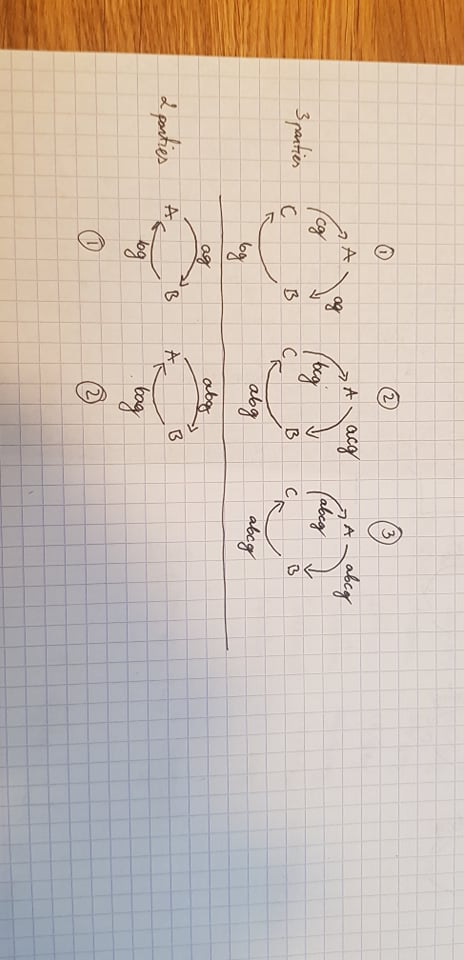
\includegraphics[scale=0.3, angle=90]{dh.jpg}
    \caption{Diffie-Hellman key exchanges.}
\end{figure}


%----------------------------------------------------------------------------------------
%	2.2 TASK 2
%----------------------------------------------------------------------------------------

\section{2.1 Task 2 - Block ciphers} 
Alice sends message m to Bob, encrypted with a block cipher. 
m is split into 6 blocks of equal length 
$m = m_0||m_1||m_2||m_3||m_4||m_5$ and encrypted using DES. 
In transmission one bit of the ciphertext $c_2$ changes its value.
\\Bob decrypts and gets
message $m^{'} = m^{'}_0||m^{'}_1||m^{'}_2||m^{'}_3||m^{'}_4||m^{'}_5$. 
\\Please, explain to 
Bob how many bits are expected to be wrong in each block $m^{'}_i$
if Alice used ECB or CBC mode.
\\\\
Electronic codebook (ECB) cipher mode.
\\
Since in ECB the only method used is confusion, then other blocks would not be affected by the single bit change inside
the message m. 
\begin{figure}[H]
    \centering
    \label{fig:ecb_decrypt}
    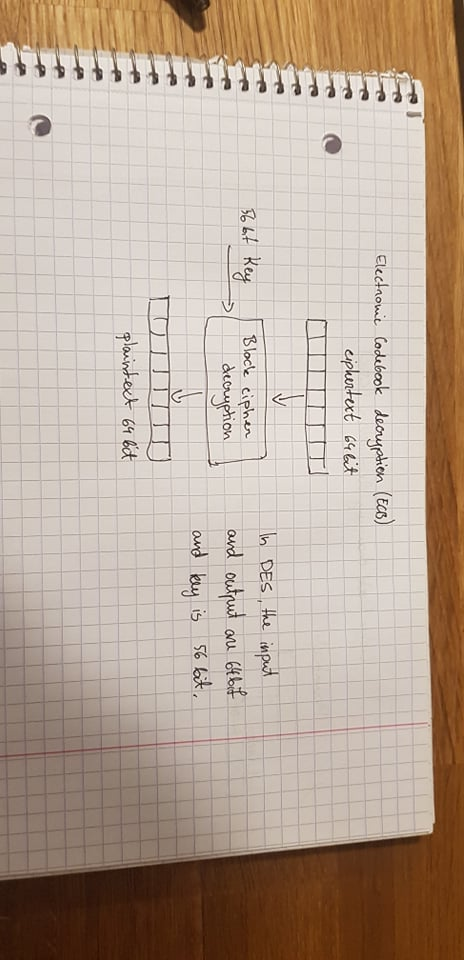
\includegraphics[scale=0.5, angle=90]{ecb_decrypt.jpg}
    \caption{ECB decrypt}
\end{figure}
Hence only a single bit will be incorrect in the final message. The incorrect bit will occur in a single decryption block.
\pagebreak
Cipher block chaining (CBC) cipher mode.\\
In CBC both diffusion and confusion are used. Meaning an incorrect bit will cause a cascade of incorrect bits
on the condition that the invalid bit is not in the final decryption block which would mean that bit would be the only invalid bit.
The closer the invalid bit is to the starting block the more bits are influenced.
If the invalid bit is in the first block. Then in our example a single bit in every block would be incorrect, meaning
there could be 1 - 6 invalid bits in a 6 block CBC cipher.
\begin{figure}[H]
    \centering
    \label{fig:cbc_decrypt}
    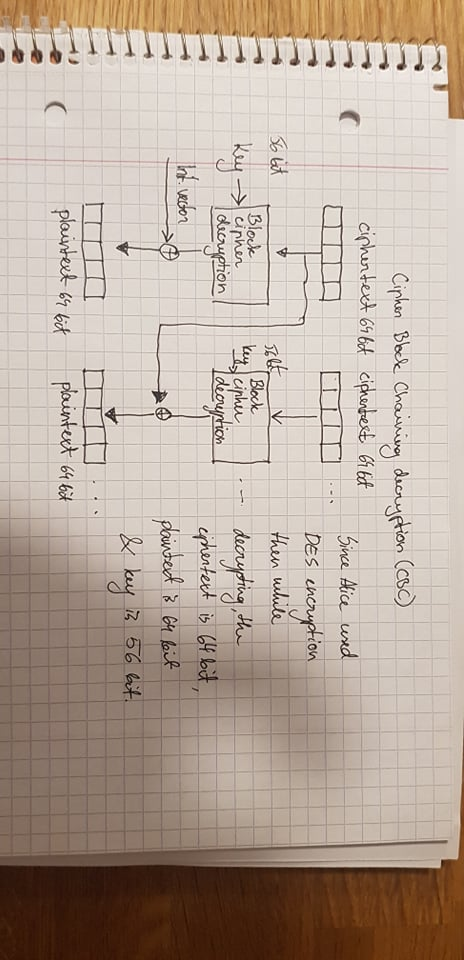
\includegraphics[scale=0.5, angle=90]{cbc_decrypt.jpg}
    \caption{CBC decrypt.}
\end{figure}


\pagebreak
\section{2.3 Task 3 - Security definitions and proofs} 
Show that OTP (one time pad) in CBC mode does not satisfy the security definition, by describing an attack.
We send $m_1 and m_2$ to the Challenger and get back c. The adversary would take c and check if conducting modulo arithmetic
with the sent messages and recieved IV gives us back the recieved c or not.
$c_2 = m_{0_0} \oplus m_{0_1} \oplus IV$ or $c_2 = m_{1_0} \oplus m_{1_1} \oplus IV$ which ever matches c. So it seems 
this advesary has an non-neglible advantage.
\begin{figure}[H]
    \centering
    \label{fig:cbc_encrypt}
    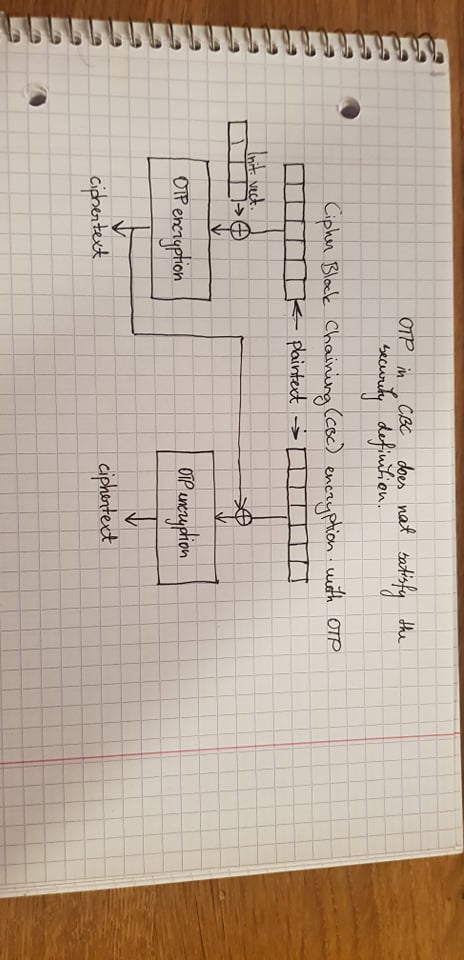
\includegraphics[scale=0.5, angle=90]{cbc_enc.jpg}
    \caption{CBC encrypt mode with OTP.}
\end{figure}

\section{2.4 Task 4 O-notation}

Show that 
\[O(n^3)= 11n^3 +4n^2 + 9n - 36\]
\[11n^3 +4n^2 + 9n - 36 \leq  c \cdot n^3 \]
\[c = 12\]
\[n^3 - 4n^2 - 9n + 36 \geq 0\]
\\Show that 
\[O(n^4) = 5n^4 - 4n^{2} - 4\]
\[5n^4 - 4n^{2} - 4\leq  c \cdot n^4 \]
\[c = 6\]
\[n^4 + 4n^{2} + 4 \geq 0\]

\end{document}